\section{Gauge Freedom in the Landau Problem}
\label{sec:landau}

\subsection{The Landau Problem}

Next we investigated the degrees of gauge freedom present in the Landau problem
of a uniform everywhere magnetic field, $\mathbf{B} = B \basis{z}$. Of
particular interest is how the ground state wavefunction gains the freedom from
the choice of gauge. This is examined explicitly for the straight and circular
gauges, with particular emphasis placed on the degeneracy of the circular gauge
ground state due to the degeneracy function $f(x,y)$ that appears in the
wavefunction solution, free to be any analytic function.

\subsection{The Straight Gauge}

In the straight gauge, $\mathbf{A} = Bx\basis{y}$, the ground state solution for
the wavefunction is
\begin{align}
    \Psi_{s,0}(x,t) = \mathcal{N} e^{- \frac{1}{2} \mymu x^2} e^{-i \frac{1}{2}
        \hbar \Omega t},
\end{align}
where $\mathcal{N}$ is a normalisation factor and $\Omega = \frac{qB}{m}$ is the
angular frequency \cite{murayama}. This ``Gaussian ridge''
wavefunction is plotted in Figure \ref{subfig:straight-wavefunction},
illustrating its invariance to translations in the $y$ direction.

The associated probability density and phase of the wavefunction are
\begin{align}
    \rho = \mathcal{N}^2 e^{- \mymu x^2} \\
    \mathrm{and}~ \theta = - \frac{1}{2} \hbar \Omega t,
\end{align}
and the probability current, as plotted in Figure \ref{subfig:straight-current},
is
\begin{align}
    \mathbf{J}_s &= \frac{\hbar}{m} \mathcal{N}^2 e^{- \mymu x^2} \left(
        \nabla \left\{ -\frac{1}{2} \hbar \Omega t \right\} - \frac{q}{\hbar} B
        x \basis{y} \right) \\
    &= - \Omega \mathcal{N}^2 e^{- \mymu x^2} x\basis{y} ~\mathrm{as}~
        \nabla \left\{ -\frac{1}{2} \hbar \Omega t \right\} = 0.
\end{align}

Importantly, this wavefunction is invariant under translations of both $y$, due to the choice of gauge. In a sense, the gauge freedom we have in
choosing $\mathbf{A}$ gives us the symmetry in $\Psi_{s,0}$.

\begin{figure}
    \centering
    \begin{subfigure}{0.45\linewidth}
        \centering
        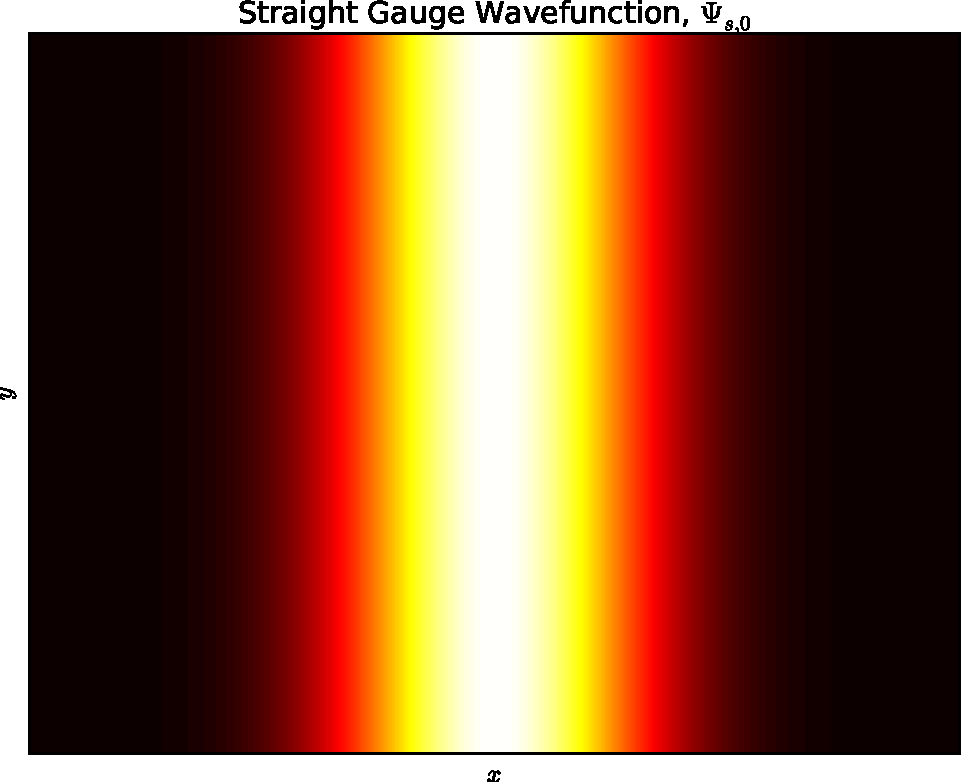
\includegraphics[width=\linewidth]{straight-gauge-wavefunction}
        \caption{The modulus of the ground state wavefunction. Note the
            independence of the $y$ coordinate.}
        \label{subfig:straight-wavefunction}
    \end{subfigure}
    \begin{subfigure}{0.45\linewidth}
        \centering
        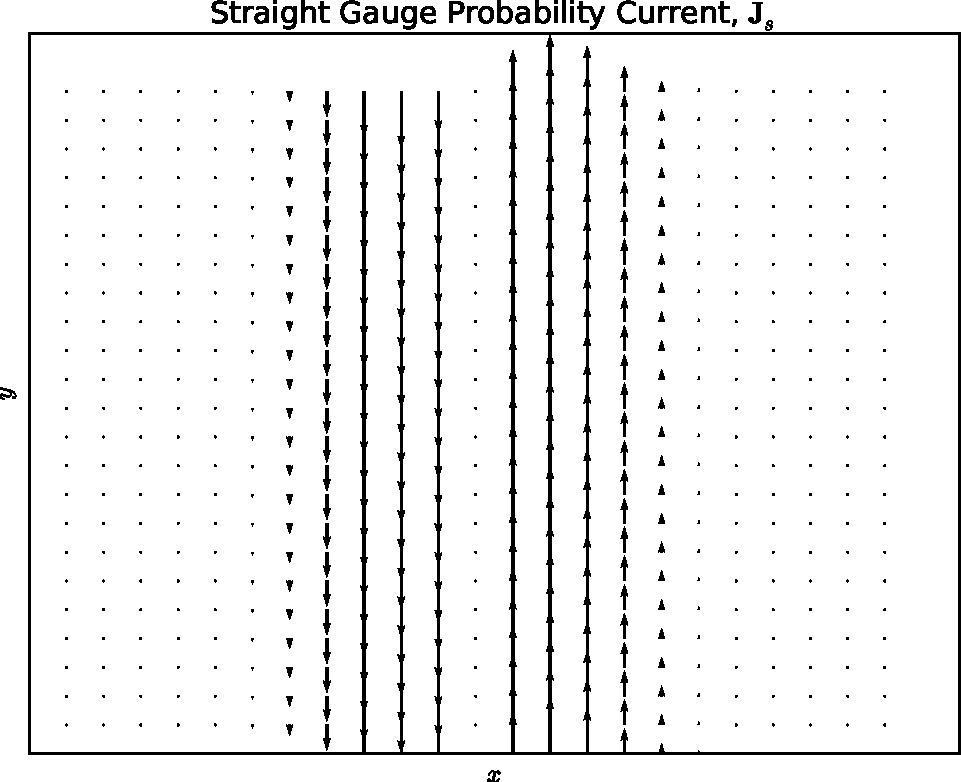
\includegraphics[width=\linewidth]{straight-gauge-current}
        \caption{The ground state probability current. Note that it points
            always in the $y$ or $-y$ directions.}
        \label{subfig:straight-current}
    \end{subfigure}
    \caption{Ground state and probability current solutions to the Landau
    problem in the straight gauge, $\mathbf{A} = Bx\basis{y}$.}
    \label{fig:straight}
\end{figure}

\subsection{The Circular Gauge}

When using the circular gauge, $\mathbf{A} = \frac{1}{2} B \left( x \basis{y} -
y \basis{x} \right)$, the ground state wavefunction is a two dimensional
``Gaussian bulge'':
\begin{align}
    \Psi_{c,0}(x, y, t) = \mathcal{N} f(x,y) e^{- \frac{1}{4} \mymu \left( x^2 +
        y^2 \right)} e^{-i \frac{1}{2} \hbar \Omega t},
\end{align}
where $f(x,y)$ is any complex analytic function \cite{murayama}. Figure
\ref{subfig:circular-wavefunction} shows that whereas previously the
wavefunction was invariant to translations in the $y$ directions, now the
wavefunction is invariant to rotations about the origin; choosing the gauge is
equivalent to choosing the symmetry of the resulting wavefunction.

If we write the function $f(x,y)$ in terms of the modulus and phase as
$f(F,\phi) = Fe^{i \phi}$, then this wavefunction has probability density
\begin{align}
    \rho = \mathcal{N}^2 F^2 e^{- \frac{1}{2} \mymu \left( x^2 + y^2 \right)},
    \label{eqn:circular-density}
\end{align}
and the probability current corresponding to this wavefunction, as plotted in
Figure \ref{subfig:circular-current}, is
\begin{align}
    \mathbf{J}_c(f) = F^2 \mathcal{M} e^{- \mu
        \left( x^2 + y^2 \right)} \left( \nabla \phi - \mu \left(
        x\basis{y} - y\basis{x} \right) \right),
\end{align}
where $\mathcal{M} = \frac{\hbar}{m} \mathcal{N}^2$ and $\mu = \frac{1}{2}
\mymu$ for brevity.

\begin{figure}
    \centering
    \begin{subfigure}{0.45\linewidth}
        \centering
        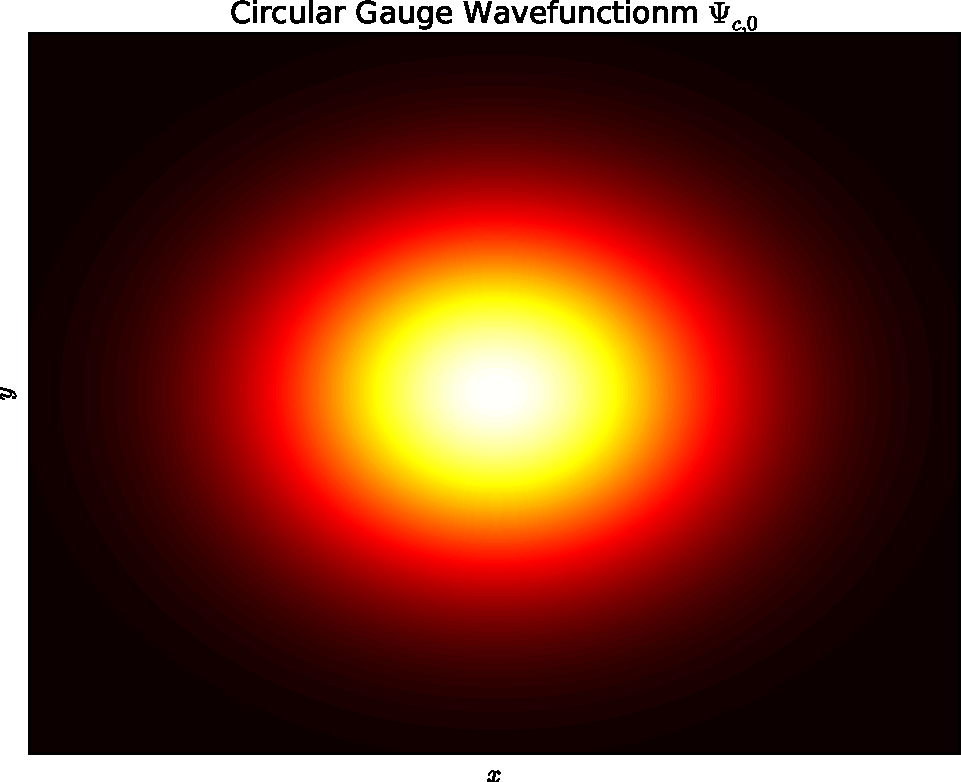
\includegraphics[width=\linewidth]{circular-gauge-wavefunction}
        \caption{The modulus of the ground state wavefunction solution to the
            Landau problem when using the circular gauge.}
        \label{subfig:circular-wavefunction}
    \end{subfigure}
    \begin{subfigure}{0.45\linewidth}
        \centering
        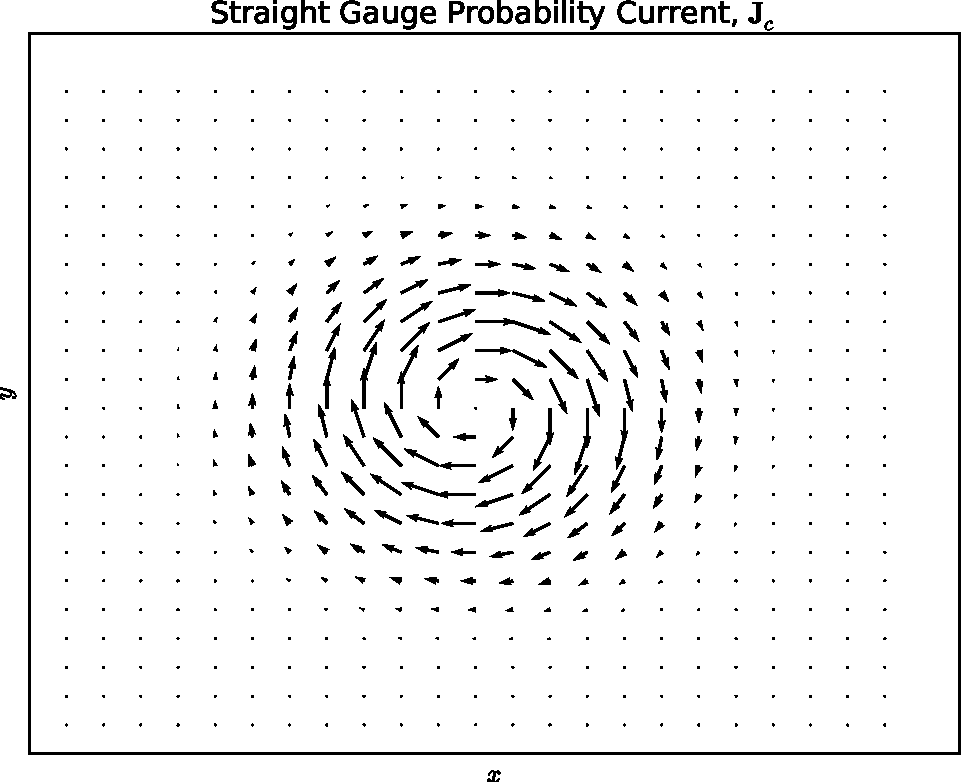
\includegraphics[width=\linewidth]{circular-gauge-current}
        \caption{The probability current corresponding to the ground state solution
            of the Landau problem, using the circular gauge.}
        \label{subfig:circular-current}
    \end{subfigure}
    \caption{The ground state wavefunction and probability current for the
        Landau problem using the circular gauge, $\mathbf{A} = \frac{1}{2} B
        \left( x\basis{y} - y\basis{x} \right)$.}
    \label{fig:circular}
\end{figure}

Note how the probability current spins clockwise around the central peak of the
wavefunction; indeed, the current points at all times parallel or anti-parallel
to the symmetry of the wavefunction; the straight gauge wavefunction has $y$
translation invariance, and $\mathbf{J}_s$ points always in the $\pm y$
direction, while the circular gauge wavefunction has rotational invariance, and
$\mathbf{J}_c$ always points tangentially.

\subsection{Equivalence of probability currents}

If we choose $f(x,y)$ to be
\begin{align}
    f_s(x,y) &= e^{- \frac{1}{4} \mymu \left( x + i y \right)^2} \\
             &= e^{- \frac{1}{4} \mymu \left( x^2 - y^2 \right)}
                e^{-i \frac{1}{2} \mymu xy},
\end{align}
then the modulus and phase of the wavefunction are
\begin{align}
    F_s &= e^{- \frac{1}{4} \mymu \left( x^2 - y^2 \right)} \\
    \mathrm{and}~ \phi_s &= -\frac{1}{2} \mymu xy.
\end{align}
Thus, the probability current is
\begin{align}
    \mathbf{J}_c(f_s)
    &= F_s^2 \mathcal{M} e^{- \mu \left( x^2 + y^2 \right)}
       \left( \nabla \phi_s - \mu \left( x\basis{y} -
       y\basis{x} \right) \right) \\
    &= e^{- \mu \left( x^2 - y^2 \right)} \mathcal{M} e^{- \mu \left( x^2 + y^2
       \right)} \left( \nabla \left\{ - \mu xy \right\} - \mu \left( x\basis{y} - y
       \basis{x} \right) \right) \\
    &= - \mathcal{M} \mu e^{- \frac{1}{2} \frac{M
       \Omega}{\hbar} x^2} \left( \nabla \left\{ xy \right\} + x\basis{y} -
       y\basis{x} \right) \\
    &= - \mathcal{M} \mu e^{- \frac{1}{2} \frac{M
       \Omega}{\hbar} x^2} \left( x\basis{y} + y\basis{x} + x\basis{y} -
       y\basis{x} \right) \\
    &= - \Omega \mathcal{N}^2  e^{- \frac{1}{2} \frac{M \Omega}{\hbar} x^2}
       x\basis{y} \\
       &= \mathbf{J}_s.
\end{align}

This means that one can choose a particular value of $f(x,y)$ for which the
circular gauge reduces to the straight gauge. This raises the interesting
question of whether all values of $f(x,y)$ are permitted by continuity, and
whether the $\mathbf{J}_c(f)$ currents form a basis for all the possible
$\mathbf{J}$ values.

\subsection{Locking the analyticity of $f(x,y)$ to continuity}

Here we demonstrate that all $f(x,y)$, provided only they are analytic, produce
a respectable probability current. In other words, the associated
probability current $\mathbf{J}_c(f)$ satisfies the continuity equation
(Equation \ref{eqn:continuity}). Here $\Psi_{c,0}(x, y, t)$ has $\rho =
\mathcal{N}^2 F^2 e^{- \frac{1}{2} \mymu \left( x^2 + y^2 \right)}$ as per
Equation \ref{eqn:circular-density}. Thus
\begin{align}
    \dot \rho &= \frac{\partial}{\partial t} \left( \mathcal{N}^2 F^2 e^{-
        \frac{1}{2} \mymu \left( x^2 + y^2 \right)} \right) \\
    &= 0,
\end{align}
and the continuity equation is simply
\begin{align}
    \nabla \cdot \mathbf{J}_c(f) = 0.
\end{align}

To demonstrate this, we first make two observations of the consequences of the
analyticity of $f(x,y)$.

Firstly, the real and imaginary parts of $f(x,y)$, $f_R$ and $f_I$, are harmonic
and obey Cauchy-Riemann (CR);
\begin{align}
    \nabla^2 f_R &= \partial_x^2 f_R + \partial_y^2 f_R = 0 \\
    \mathrm{and}~ \nabla^2 f_I &= \partial_x^2 f_I + \partial_y^2 f_I = 0; \\
    \partial_x f_R &= \partial_y f_I \\
    \mathrm{and}~ \partial_y f_R &= - \partial_x f_I
\end{align}

Secondly, for any function $g(z)$, if $g(z)$ is analytic on $\mathbb{C}$, then the
principal branch of $\logg{g(z)}$ is analytic on $\mathbb{C} \setminus \left\{
g(z) \in \mathbb{R} : g(z) \le 0 \right\}$ \cite{laptev,o-farrill}.

Thus, if we take the principal branch of $\log$, and discard the negative real
line $f(x,y) \in \mathbb{R}:f(x,y) \le 0$, then $\logg{f(x,y)}$ is also
analytic, and the real and imaginary parts of this are also harmonic and obey
CR;
\begin{align}
    \logg{f(x,y)} &= \logg{F} + i \phi, ~\mathrm{therefore} \\
    \nabla^2 \logg{F} &= 0 \\
    \mathrm{and}~ \nabla^2 \phi &= 0 ~\mathrm{by~harmonicity,~while} \\
    \partial_x \logg{F} &= \partial_y \phi
    \label{eqn:log-cr-1} \\
    \mathrm{and}~ \partial_y \logg{F} &= - \partial_x \phi ~\mathrm{by~CR}.
    \label{eqn:log-cr-2}
\end{align}

A consequence of this is that $\nabla F \cdot \nabla \phi = 0$, as can be
shown simply in components;
\begin{align}
    \nabla F \cdot \nabla \phi
        &= \colvec{\partial_x F}{\partial_y F}{0} \cdot
        \colvec{\partial_x \phi}{\partial_y \phi}{0} \\
        &= \colvec{\partial_x F}{\partial_y F}{0} \cdot
        \colvec{- \partial_y \logg{F}}{\partial_x \logg{F}}{0} \\
        &= \frac{1}{F} \colvec{\partial_x F}{\partial_y F}{0} \cdot
        \colvec{- \partial_y F}{\partial_x F}{0} \\
        &= 0
\end{align}

Using these facts, the divergence of $\mathbf{J}_c$ can be expressed as
\begin{align}
    \div{J}_c - -2\mu F^2 \mathcal{M} e^{-\mu\left(x^2 + y^2\right)} \left[
        \nabla \logg{F} \cdot \left( x\basis{y} - y\basis{x} \right) + \nabla
        \phi \cdot \left( \mathbf{x} + \mathbf{y} \right) \right].
    \label{eqn:div-j}
\end{align}

\Cref{eqn:log-cr-1,eqn:log-cr-2} allow us to express $\nabla \phi$ as
\begin{align}
    \nabla \phi = \basis{z} \times \nabla \logg{F},
\end{align}
which means that by the cyclic permutation of the scalar product
\begin{align}
    \nabla \phi \cdot \left( \mathbf{x} + \mathbf{y} \right)
    &= \left( \basis{z} \times \nabla \logg{F} \right) \cdot \left( \mathbf{x} +
        \mathbf{y} \right) \\
    &= \nabla \logg{F} \cdot \left[ \left( \mathbf{x} + \mathbf{y} \right)
        \times \basis{z} \right] \\
    &= - \nabla \logg{F} \cdot \left( x\basis{y} - y\basis{x} \right).
\end{align}

Thus, the bracketed term in \Cref{eqn:div-j} cancels and the divergence of
$\mathbf{J}_c$ is zero for all analytic functions $f(x,y)$.

\subsection{Strictness of $\mathbf{J}$ versus $f(x,y)$}

So we have established that for every $f(x,y)$ there corresponds a
divergenceless $\mathbf{J}_c(f)$, so next we consider whether any given
$\mathbf{J}$ has a corresponding analytic function $f(x,y)$. This is equivalent
to asking whether the condition of analyticity on $f(x,y)$ is stronger than or
equivalent to the condition of divergencelessness of $\mathbf{J}$.

An important result of complex analysis is that any analytic real function can
be extended or analytically continued into an analytic function on the entire
complex plane. This means that any complex function can be uniquely specified by
its value on the real axis. Thus, any analytic function $f(x,y)$ is entirely
determined by the value along the real axis, $f(x,0)$, and $f(x,y)$ is
essentially two functions $f_R$ and $f_I$ of one variable, $x$.

The condition of divergencelessness on the probability current means that $J_x =
- J_y$. Thus $\mathbf{J}$ is essentially one function of two variables, $x$ and
$y$. In this plane, this single function representing the divergenceless
probability current can have any value; it is unrestrained.

A divergenceless quantity can therefore still take unique values across the
whole $x,y$ plane, whereas an analytic function is entirely uniquely determined
by just the $y = 0$ line. Therefore, the condition of analyticity is more
stringent than the condition of continuity; every analytic $f(x,y)$ has a
corresponding divergenceless $\mathbf{J}_c$, but not every divergenceless
$\mathbf{J}$ has a corresponding $f(x,y)$.
